\documentclass[11pt]{article}
\usepackage[UTF8]{ctex}
\usepackage[a4paper]{geometry}
\geometry{left=2.0cm,right=2.0cm,top=2.5cm,bottom=2.5cm}

\usepackage{caption}
\usepackage{paralist}
\usepackage{enumitem}
\setenumerate[1]{itemsep=0pt,partopsep=0pt,parsep=0pt,topsep=0pt}
\setitemize[1]{itemsep=2pt,partopsep=0pt,parsep=\parskip,topsep=2pt}
\usepackage{comment}
\usepackage{booktabs}
\usepackage{graphicx}
\usepackage{float}
\usepackage{diagbox}
\usepackage{amsmath,amsfonts,graphicx,amssymb,bm,amsthm}
%\usepackage{algorithm,algorithmicx}
\usepackage[ruled, linesnumbered]{algorithm2e}
% \usepackage[linesnumbered]{algorithm2e}
\usepackage[noend]{algpseudocode}
\usepackage{fancyhdr}
\usepackage{tikz}
\usepackage{graphicx}
\usetikzlibrary{arrows,automata}
\usepackage{hyperref}
\usepackage{extarrows}
% 这是一些字体选项
\usepackage{helvet}
% \usepackage{mathpazo}
\usepackage{fontspec}
% \setmainfont{Times New Roman}
% \setmainfont{Comic Sans MS} % 比较fancy的字体
% \setmainfont{Avenir}
% \setmainfont{Palatino}

\setlength{\headheight}{14pt}
\setlength{\parindent}{0 in}
\setlength{\parskip}{0.5 em}


\newtheorem{theorem}{Theorem}
\newtheorem{lemma}[theorem]{Lemma}
\newtheorem{proposition}[theorem]{Proposition}
\newtheorem{claim}[theorem]{Claim}
\newtheorem{corollary}[theorem]{Corollary}
\newtheorem{definition}[theorem]{Definition}
\newtheorem*{definition*}{Definition}

\newenvironment{problem}[2][Problem]{\begin{trivlist}
\item[\hskip \labelsep{\bfseries#1}\hskip\labelsep{\bfseries#2.}]}{\hfill$\blacktriangleleft$\end{trivlist}}
\newenvironment{answer}[1][Answer]{\begin{trivlist}
\item[\hskip \labelsep{\bfseries\itshape#1.}\hskip \labelsep]}{\hfill$\lhd$\end{trivlist}}

\newcommand\E{\mathbb{E}}
\newcommand\per{\mathrm{per}}
% chktex-file 44
% \renewcommand{\familydefault}{\sfdefault}

\title{Homework \#1}
\usetikzlibrary{positioning}

\begin{document}
\captionsetup[figure]{labelfont={bf},name={Fig.},labelsep=period}
\kaishu

\pagestyle{fancy}
\lhead{\CJKfamily{zhkai} Peking University}
\chead{}
\rhead{\CJKfamily{zhkai} Algorithm Design and Analysis (Honor Track)}

\begin{center}
    {\LARGE \bf Homework 2}\\
    {Name: 方嘉聪\ \  ID: 2200017849}            % Write down your name and ID here.
\end{center}

\begin{problem}{1 (Textbook 2.7)}
    设$A$是含有$n$个元素的数组, 如果元素$x$在$A$中出现的次数大于$n/2$, 则称$x$是$A$的主元素.
    \begin{enumerate}[label =(\arabic*)]
        \item 如果$A$中的元素是可以排序的, 设计一个$O(n \log n)$时间的算法判断$A$是否有主元素.
        \item 对于$(1)$中可排序的数组, 能否设计一个$O(n)$时间的算法.
        \item 如果$A$中元素只能进行“是否相等”的测试, 但无法排序, 设计一个算法判断$A$是否有主元素.
    \end{enumerate}
\end{problem}
\begin{answer}
    \begin{enumerate}[label = (\arabic*)]
        \item 算法一: \textbf{基于排序的算法}. 先对数组进行排序, 再遍历数组记录出现次数最多的元素, 最后检查是否为主元素.
        时间复杂度$T(n) = O(n \log n) + O(n) + O(n)= O(n \log n), $具体思路见下:
        \begin{algorithm}\footnotesize
            \caption{\textbf{Sort and Count(By Vote)}}
            \KwIn{An array $A$ of size $n$}
            \KwOut{Whether $A$ has a majority element}
            Sort the array $A$ in $O(n \log n)$ time. \\
            Initialize $count = 1$, $major = A[0]$.\\
            Find the maximum number of the same element in $A$ \textbf{by vote} in $O(n)$ time.\\
            Check the number of the $major$ in $A$ in $O(n)$ time.\\
        \end{algorithm}
        \\算法二: \textbf{基于分治的算法}. 首先证明下面一个引理:
        \begin{lemma}
            如果数组$A$有主元素, 则数组$A$的子数组$A[0:n/2]$和$A[n/2:n]$中至少有一个有主元素.
        \end{lemma} 
        \begin{proof}
            设数组$A$的主元素为$x$, $L_1 = A[0:n/2], L_2 = A[n/2: n]$, 设$L_1$ 中含有$x$的个数为$i$, $L_2$中含有$x$的个数为$j$,
            如果$i \le \left\lfloor n/2 \right\rfloor, j \le \left\lceil n/2 \right\rceil$, 那么有$i + j \le n$, 矛盾. 因此至少有一个子数组中含有主元素.
        \end{proof}
        \begin{algorithm}\footnotesize
            \caption{\textbf{Divide and Conquer}}
            \KwIn{An array $A$ of size $n$}
            \KwOut{the majority element $x$ and whether $A$ has a majority element}
            \uIf{$n = 1$}{
                \Return{$A[0]$, True}
            }
            $m_1 \leftarrow DivideAndConquer(A[0:n/2])$, $m_2 \leftarrow DivideAndConquer(A[n/2:n])$\\
            \uIf{$m_1 = m_2$}{
                \Return{$m_1$, True}
            }
            \uElseIf{$m_1$ and $m_2$ don't exist}{
                \Return{None, False}
            }
            \uElse{
                check the number of $m_1$ and $m_2$(if it exists) in $A$\\
            }
        \end{algorithm}
        第9行的检查操作可以在$O(n)$时间内完成, 因此整个算法的时间复杂度为$T(n) = 2T(n/2) + O(n) = O(n \log n)$.
    \item 先证明一个引理:
    \begin{lemma}
        $A$ 中的主元素一定是中位数.
    \end{lemma}
    \begin{proof}
        假设主元素不是中位数, 那么在有序的数组中主元素只能分布在中位数的一侧, 那么主元素的个数一定不超过$n/2$, 矛盾.
    \end{proof}
    \begin{algorithm}
        \caption{\textbf{Find Median and Check}}
        \KwIn{An array $A$ of size $n$}
        \KwOut{Whether $A$ has a majority element}
        Find the median of $A$ in $O(n)$ time.\\
        Check the number of the median in $A$ in $O(n)$ time.\\
    \end{algorithm}
    第1行可以使用课上证明的\textbf{确定性快速选择算法}.总的时间复杂度$T(n) = O(n) + O(n) = O(n)$.
    \item 采用两两比较并将不同的元素删除的方法(\textbf{类似课上提及的芯片测试算法}), 最后剩下的元素即为主元素. 时间复杂度为$O(n)$.伪代码如下:
    \begin{algorithm}
        \caption{\textbf{Delete Different Elements}}
        \KwIn{An array $A$ of size $n$}
        \KwOut{Whether $A$ has a majority element}
        \While{$|A| > 1$}{
            Group the elements in $A$ in pairs\\
            \For{each group}{
                \uIf{the two elements are different}{
                    Delete the two elements.
                }
                \uElse{
                    Keep one element.
                }
            }
        }
        Check the remaining element in $A$ in $O(n)$ time.\\
    \end{algorithm}
    \\时间复杂度$T(n) = T(\frac{n}{2}) + O(n) \implies T(n) = O(n)$.
    \end{enumerate}
\end{answer}

\begin{problem}{2 (Textbook 2.27)}
    如下图所示, 城市街道都是水平或垂直分布, 有$m+1$条, 不妨设任何两个相邻位置之间的距离都为$1$. 
    在街道的十字路口有$n$的商店, 图中$n=3, m=8$, 三个商店的位置坐标分别为$(2,4), (5,3), (6,6)$. 
    现在需要在某个路口位置见一个合用的仓库. 若仓库选择$(3,5)$的位置, 那么这3个商店到仓库的路程(只能沿街道行进)
    总长至少为10. 请设计一个算法找到仓库的最佳位置, 使得所有商店到仓库路程的总长最小.
    % \begin{figure}[H]
    %     \centering
    %     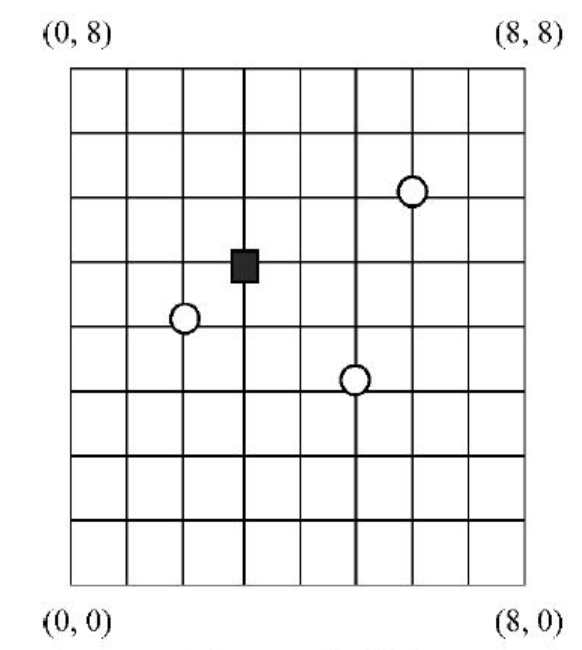
\includegraphics[width = 0.25\textwidth]{images/problem2.png}
    %     \caption{街道图}
    % \end{figure}
\end{problem}
\begin{answer}
    不妨设$n$个点的坐标为$(x_1, y_1), (x_2, y_2), \cdots , (x_n, y_n)$, 那么目标为
    \begin{align*}
        \min_{(x, y)} \sum_{i = 1}^{n} |x - x_i| + |y - y_i|
    \end{align*}
    注意到横纵坐标是独立的, 因此可以分别求解. 不妨先考虑横坐标, 问题转化为
    \begin{align*}
        \min_{x} \sum_{i = 1}^{n} |x - x_i|
    \end{align*}
    由于$|x - x_i|$是关于$x$的绝对值函数, 因此可以得到$x$的最优解为$x = x_{(n+1)/2}$, 即中位数. 同理, $y$的最优解为$y = y_{(n+1)/2}$. 因此仓库的最佳位置为$(x_{(n+1)/2}, y_{(n+1)/2})$.
    那么只要使用\textbf{\underbar{快速选择算法}}即可在$O(n)$时间内找到中位数, 因此整个算法的时间复杂度为$O(n)$.
\end{answer}

\begin{problem}{3 (Forces Between Particles)}
    You guys have learned about how to compute the electrostatic forces between two charged particles in high 
    school physics. Consider a case where we have particles at points $\{1, 2, \cdots , n\}$ on the real axis, 
    and the particle at point $j$ has charge $q_j$ (the charge can be either positive or negative). 
    By Coulomb’s law, the total force on each particle $j$ is:
    \begin{align*}
        F_j = \sum_{i < j}\frac{C q_i q_j}{(j-i)^2} - \sum_{i > j}\frac{C q_i q_j}{(j-i)^2}
    \end{align*}
    where $C$ is a given constant (the Coulomb constant). Design an algorithm that
    computes all the forces $F_j, j = 1, 2, \cdots, n$ in $O(n \log n)$ time.
\end{problem}
\begin{answer}
    基本思路: 找到两个向量$\alpha$和$\beta$, 使得$\alpha$和$\beta$的卷积的第$n+j+1$个分量为
    \begin{align} 
        (\alpha * \beta)[n+j+1] := \sum_{i<j} \frac{q_i}{(j-i)^2} + \sum_{i>j} \frac{-q_i}{(j-i)^2}, (j \in \{1, 2, \cdots, n\})
        \label{a}
    \end{align}
    而后我们调用$FFT$算法计算卷积, 最后再对对应分量乘上$C q_j$即可得到$F_j$. 
    \\事实上我们考虑
    \begin{align*}
        \alpha = \left(q_1, q_2, \cdots, q_n\right), 
        \beta = \left(-\frac{1}{n^2}, -\frac{1}{(n-1)^2}, \cdots, -1, 0, 1, \cdots, \frac{1}{(n-1)^2}, \frac{1}{n^2}\right)
    \end{align*}
    容易证明$\alpha, \beta$如上取值满足\ref{a}式. 由于$FFT$算法的时间复杂度为$O(n \log n)$, 因此整个算法的时间复杂度为$O(n \log n)$.


\end{answer}

\begin{problem}{4 (Median of Medians)}
    The $Quickselect(A, k) algorithm$ for finding the $k-th$ smallest element in an unsorted array $A$
    picks an arbitrary pivot, then partitions the array into three pieces: the elements less than the 
    pivot, the elements equal to the pivot, and the elements that are greater than the pivot. 
    It is then recursively called on the piece of the array that still contains the $k-th$ smallest element.
    \begin{enumerate}[label = (\alph*)]
        \item Consider the array A = $\left[1,2,\cdots,n\right]$ shuffled into some arbitrary order. 
        What is the worst-case runtime of $Quickselect(A, n/2)$ in terms of n? Construct a sequence 
        of bad pivot choices that achieves this worst-case runtime.
        \item  The above worst case has a chance of occurring even with randomly-chosen pivots, so the worst-case time for a random-pivot Quickselect is $O(n^2)$.
        \\ Lets define a new algorithm Better-Quickselect that deterministically picks a better pivot. This pivot-selection strategy is called Median of Medians, 
        so that the worst-case runtime of Better-Quickselect(A, k) is $O(n)$.
        \begin{algorithm}
            \caption{\textbf{Median of Medians}}
            \KwIn{An array $A$ of size $n$ and an integer $k$}
            \KwOut{The $k-th$ smallest element in $A$}
            \begin{enumerate}
            \item Group the array into  $\left\lfloor \frac{n}{5}\right\rfloor$ groups of 5 elements each (ignore any leftover elements)
            \item Find the median of each group of 5 elements (as each group has a constant 5 elements, finding
            each individual median is $O(1)$)
            \item Create a new array with only the $\left\lfloor \frac{n}{5}\right\rfloor$ medians, and find the true median of this array using Better-Quickselect.
            \item Return this median as the chosen pivot.
            \end{enumerate}
        \end{algorithm}
        \\Let $p$ be the chosen pivot. Show that for least $3n/10$ elements $x$ we have that $p > x$, and that for at least $3n/10$ elements we have that $p \le x$.
        \item Show that the worst-case runtime of Better-Quickselect(A, k) using the Median of Medians strategy is $O(n)$.
        \textit{Hint: Using the Master theorem will likely not work here. Find a recurrence relation for $T(n)$, and try to use induction to show that $T (n) \le cn$ for some $c > 0$.}
    \end{enumerate}
\end{problem}
\begin{answer}
    \begin{enumerate}[label = (\alph*)]
        \item 最坏情况下的时间复杂度为$O(n^2)$, 例如: 以序列$$ \left[1,2, 3, \cdots, \frac{n}{2} - 1, n, n-1, \cdots, \frac{n}{2} + 1, n/2 \right]$$ 
        取pivot, 这样每次调用只删去了一个元素, 因此时间复杂度为$O(n^2)$.
        \item 总共分成了$n/5$份, 由于$p$是中位数的中位数, 因此$p$至少大于一半的中位数 (即至少大于$3 *(n/10) = 3n/10$个元素), 至少小于一半的中位数 (即至少小于$3n/10$个元素).
        \item 设小于$p$的元素个数为$S_1$, 大于$p$的元素个数为$S_2$, 那么$S_1 \ge 3n/10, S_2 \ge 3n/10 \implies 3n/10 \le S_1, S_2 \le 7n/10$.
        设最坏情况下时间复杂度为$T(n)$, 那么有
        \begin{align*}
            T(n) = T(\frac{n}{5}) + T(\frac{7n}{10}) + O(n)
        \end{align*}
        其中, $T(n/5)$为求中位数的中位数的时间(算法中$\left(c\right)$), $T(7n/10)$为递归调用的时间, $O(n)$为找到各组中位数的时间(算法中$\left(b\right)$).
        我们可以通过递归树的方法证明$T(n) = O(n)$.

    \end{enumerate}
\end{answer}
\begin{problem}{5 (Draw the Skyline!)}
    You are given $n$ non-vertical lines in the plane, labeled $L_1 , \cdots , L_n$ , 
    with the $i^{th}$ line specified by the equation $y = a_i x + b_i$. 
    We assume that \textbf{no three of the lines all meet at a single point}. 
    We say line $L_i$ is \textbf{uppermost} at a given $x$-coordinate $x_0$ 
    if its $y$-coordinate at $x_0$ is greater than the $y$-coordinates 
    of all the other lines at $x_0$, i.e., $a_i x_0 + b_i > a_j x_0 + b_j,  \forall j \ne i$. 
    We say line $L_i$ is \textbf{visible} if there exists some $x$-coordinate 
    at which it is uppermost. Give an algorithm that takes $n$ lines as input, 
    and in $O(n \log n)$ time returns all the visible ones.
    \begin{figure}[H]
        \centering
        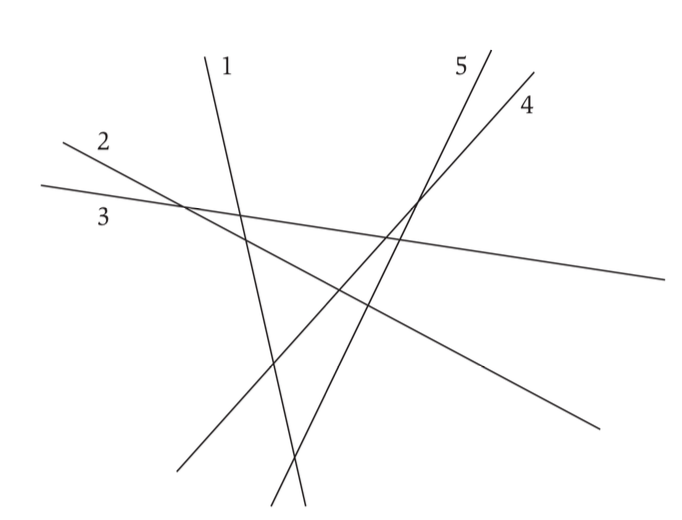
\includegraphics[width = 0.35 \textwidth]{images/skyline.png}
        \caption{An example of finding all the visible lines. All the lines except for line 2 are visible.}
    \end{figure}
\end{problem}
\begin{answer}
    大致思路: 先将所有的线段按照\textbf{斜率}$a_i$\textbf{升序排列}为$\left[L_{k_1}, L_{k_2}, \cdots, L_{k_n} \right]$, 注意到斜率最大和最小的线段一定是\textit{visible}的,
    类似的将所有线段两两分组为$\left[L_{k_1}, L_{k_n}\right], \left[L_{k_2}, L_{k_{n-1}}\right], \cdots$. 对每一组, 我们记录下交点的横坐标$x_i$以及在区间$\left(-\infty, x_i\right), \left(x_i, \infty\right)$哪条线段是\textit{uppermost}的.
    而后我们调用\textbf{\textit{Merge}}算法(思路为: 在合并两个线段集中的点的同时, 根据该点对应值的大小确定合并后的\textit{uppermost}线段)递归地将线段合并起来, 得到最终的的\textit{visible}线段. 
    \\ \textbf{\textit{Merge}}算法基本思路与伪代码见下:
    \begin{algorithm}
        \caption{\textbf{Merge}}
        \KwIn{Tow line sets $L_1, L_2$ with \textbf{sorted} intersection-points set $\{x_i\}, \{y_j\}$}
        \KwOut{One merged line sets $L$ with \textbf{sorted} intersection-points set $\{r_t\}$}
        Like merge step in merge-sort, merge $\{x_i\}$ , $\{y_i\}$ and new intersection points $\{n_s\}$ in $O(n)$.\\
        \For{$z_k$ in $\{x_i\} \cup \{y_j\} \cup {n_s}$}{ 
            \uIf{$L_1(z_k) > L_2(z_k)$}{
                Add the uppermostline of $L_1$ at $z_k$ to $L$
            }
            \uElseIf{$L_1(z_k) < L_2(z_k)$}{
                Add the uppermostline of $L_2$ at $z_k$ to $L$
            }
            \uElse{
                Add the uppermostline of $L_1$ at $z_k$ to $L$
            }
            update the intersection-points set $\{r_t\}$
        }
    \end{algorithm} \\
    这里$L_1(z_k)$表示$L_1$在$x = z_k$上对应\textit{uppermost}线段的$y$, 时间复杂度和归并排序的\textbf{Merge}操作一样, 为$O(n)$.
    下面我们来证明整个算法的时间复杂度为$O(n \log n)$.\\
    设$T(n)$为$n$个线段的\textit{visible}算法的时间复杂度, 那么有$T(n) = 2T(n/2) + O(n)$, 由\textbf{Master Theorem}可知$T(n) = O(n \log n)$.


\end{answer}

\begin{problem}{6 (Local Minima of A Chessboard)}
    Given a $n \times n$ matrix $M$, where each element $M[i][j]$,$1 \le i,j \le n$ 
    is labeled with a real number $m_{i,j}$; you may assume that 
    all these values are distinct. For each element $M[i][j]$, 
    you can determine the value $m_{i,j}$ by probing it. 
    We define that $M[i][j]$ is a \textit{local minimum iff}. 
    Its value is smaller than the values of all the adjacent 
    (left, right, up, down) elements (except for those falling out of the range of the matrix). 
    Show how to find \textbf{a local minimum} of $M$ using only $O(n)$ probes to the elements of M.
    
\end{problem}
\begin{answer}
    基本思路, 先从中间行列找到最小值$m$, 如果是\textit{local minimum}, 那么返回$m$, 
    否则, 选择$m$所在的行或列中最小的值, 递归地在这一值所在的象限调用上述算法, 直到找到\textit{local minimum}.
    伪代码如下:
    \begin{algorithm}
        \caption {\textbf{Find Local Minimum}}
        \KwIn{A $n \times n$ matrix $M$}
        \KwOut{A local minimum of $M$}
        Find the minimum value $m$ in the middle row and middle column of $M$ in $O(n)$ time.\\
        \uIf{$m$ is a local minimum}{
            \Return{$m$}
        }
        \Else{
            \tcp{Find the minimum value $m'$ in the row or column of $m$ in $O(n)$ time.}
            \textcolor{red}{Find the minimum value $m'$ in nerighbourhood of $m$.}\\
            \uIf{$m'$ is a local minimum}{
                \Return{$m'$}
            }
            \Else{
                Recursively call \textbf{Find Local Minimum} on the submatrix of $M$ that contains $m'$.
            }
        }
    \end{algorithm}
    \\时间复杂度分析: 注意到每次矩阵大小变为原来的$1/2$, 因此时间复杂度为$T(n) = T(n/2) + cn $, 那么由主定理有$ T(n) = O(n)$.
\end{answer}
    
\end{document}